
Para poder empezar la descripción primero hay que presentar una explicación del vocabulario básico. Lo cierto es que acerca de DDD y arquitecturas de software hay ingente documentación. Realizar un exposición de toda la teoría sería extenso. Como referencia fundamentar para iniciarse en el tema tomamos como referencia la devopedia\cite{devopediaDDD}. Intentar resumirlo mejor carece de valor. Este trabajo lo que intenta no es ser un manual teórico más de DDD, si no una aplicación práctica de dichos conceptos para entender en un caso real el alcance de dicha teoría. Las referencias básicas que se van a tomar son:

\begin{itemize}
    \item Domain-Driven Design: Tackling Complexity in the Heart of Software. De Eric Evans\cite{EricEvans2003DDTC}
    \item Implementing Domain-Driven Design. De Vaughn Vernon\cite{VaughnVernon2013IDD}
    \item Get Your Hands Dirty on Clean Architecture de Tom Hombergs \cite{TomHombergs2019GYHD}
\end{itemize}

Toda teoría del DDD va enfocada a desarrollar un lenguaje común a todos los interesados que intervienen en un problema y su solución: clientes, vendedores, técnicos, financieros, etc. para desarrollar ese lenguaje se divide el problema en contextos delimintados. En un ejemplo rápido afiliado en un club deportivo significa facturas, números de identificación fiscal para los financieros y para la gente de operaciones significa reserva de pistas y cancelaciones. y para los de ventas significan descuentos, promociones. Ect. El tener un lenguaje común donde todos puedan expresarse y hablar de la misma solución es el reto de este proceso. Es lo que se define como \textbf{Ubiquitous Language} o \textbf{UL}

Intentar expresar en un mismo contexto todos esos significados termina en lo que se conoce como ¨Big Ball of Mud¨ o Gran bola de barro. Los componentes de este UL se pueden apreciar en la figura  \ref{fig:DomainDrivenDesignReference}, se puede apreciar también la relación entre ellos

\begin{figure}[H]
    \centering
    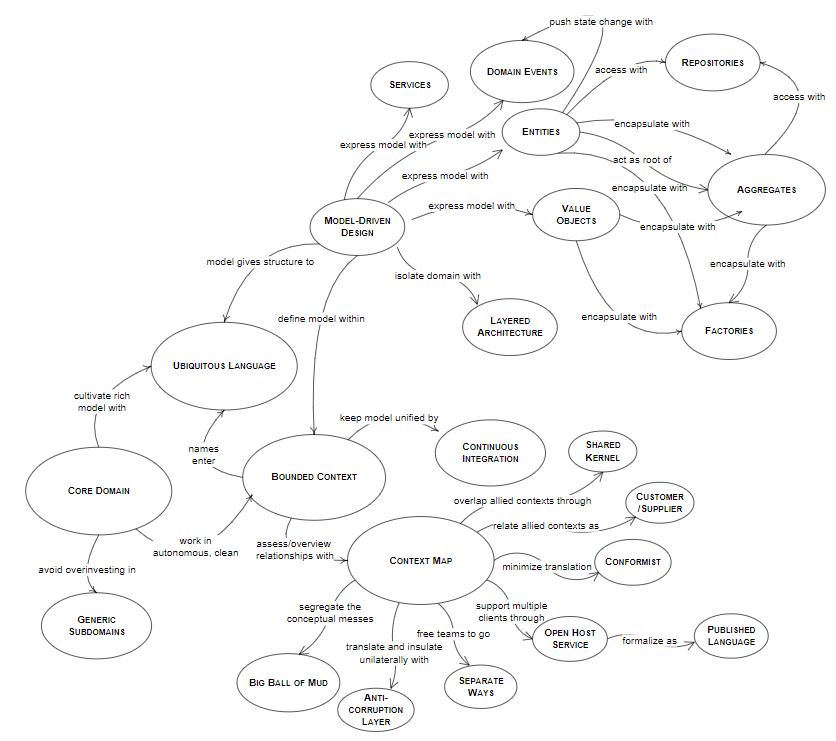
\includegraphics[height=0.5\textheight]{./part/Proyecto_ejecutivo/memoria_descriptiva/infoPreviaAntecedentes/img/DomainDrivenDesignReference}
    \caption{DomainDrivenDesignReference\cite{EricEvans2003DDTC}}\label{fig:DomainDrivenDesignReference}
\end{figure}

De todo este diagrama los conceptos en los que nos vamos a centrar

\begin{itemize}
    \item Entity: Un Objeto que tiene atributos pero principalmente definido por un identificador
    \item Value Object: Un Objeto que tiene atributos pero no identificador
    \item Domain Event: Un Objeto que define una suceso inducido por la interacción entre los componentes del dominio.
    \item Aggregate: Es un cluster de objetos tratado como una unidad. Las referencias o acciones externas sobre sus elementos siempre se hacen a través de un único elemento de este cluster conocido como Aggregate root. Tiene reglas definidas de consistencia dentro de su delimitación. External references are restricted to only one member, called the Aggregate Root.
    \item Repository: Es un mecanismo de interaccion para encapsular el acceso a tecnologías, normalmente de almacenamiento para interactuar con ellas, cuya implementación no concierne al dominio.
    \item Service: Es una funcionalidad de interacción con el dominio que garantiza la interacción con el mismo de una forma consistente
\end{itemize}

Esta definición de dominio se implementa normalmente con un paradigma de diseño conocido como arquitectura de capa. Lo que se busca es aislar esos contextos que definen nuestro dominio de implementaciones concretas ya sea para acceder al mismo o a las que accede el dominio. Por ejemplo, aislarlo de que se ejecute un servicio mediante una consola de comandos o desde una llamada http y que se guarde en una base de datos la información o se guarde en un archivo.

El tipico diagráma cuando se habla de arquitectura hexagonal es tal y como se muestra en la figura\ref{fig:hexagonalDiagram} Si bien consideramos que no tiene mucho sentido y de cara a la parte didáctica confunde, ya que el hexágono es una simple licencia estética. en el caso de existir más puertos de salida y entrada que los representados el hexágono pierde todo el sentido y cuando se enfrenta por primera vez este diagrama se tiende a intentar descifrar el sentído del hexagono.

\begin{figure}[H]
    \centering
    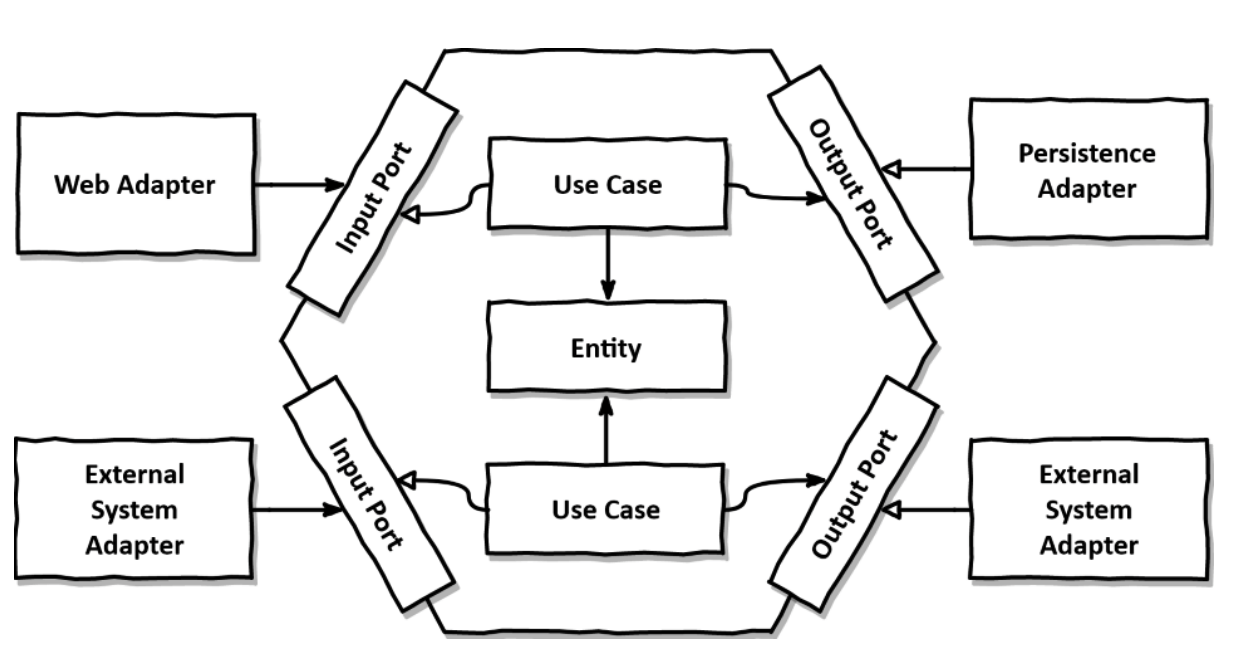
\includegraphics[height=0.3\textheight]{./part/Ejecucion/Seguimiento/CreateTaskUseCase/img/HexagonalDiagram}
    \caption{Hexagonal architecture diagram\cite{TomHombergs2019GYHD}}\label{fig:hexagonalDiagram}
\end{figure}

Vemos en este diagrama que el dominio, representado por la Entity no accede a elementos exteriores. La aplicación respresentada por los UseCase utiliza el dominio y depende de él. pero se aisla del exterior, la infraestructura obligando a utilizar interfaces a los elementos que acceden a el y obligando a implementar las interfaces definidas por la aplicación para la infraestructura que sirve para acceder al exterior de la aplicación.

En el diagrama \ref{fig:layers} podemos ver simplificado que el objetivo es que la dependencia de las capas, expresada por las flechas, sea siempre de fuera hacia adentro. Queremos preservar del cambio el interior y exponer al cambio el exterior. Separar lo propenso al cambio de lo que no. El UL de los detalles de implementación que tienen su propio lenguaje.

\begin{figure}[H]
    \centering
    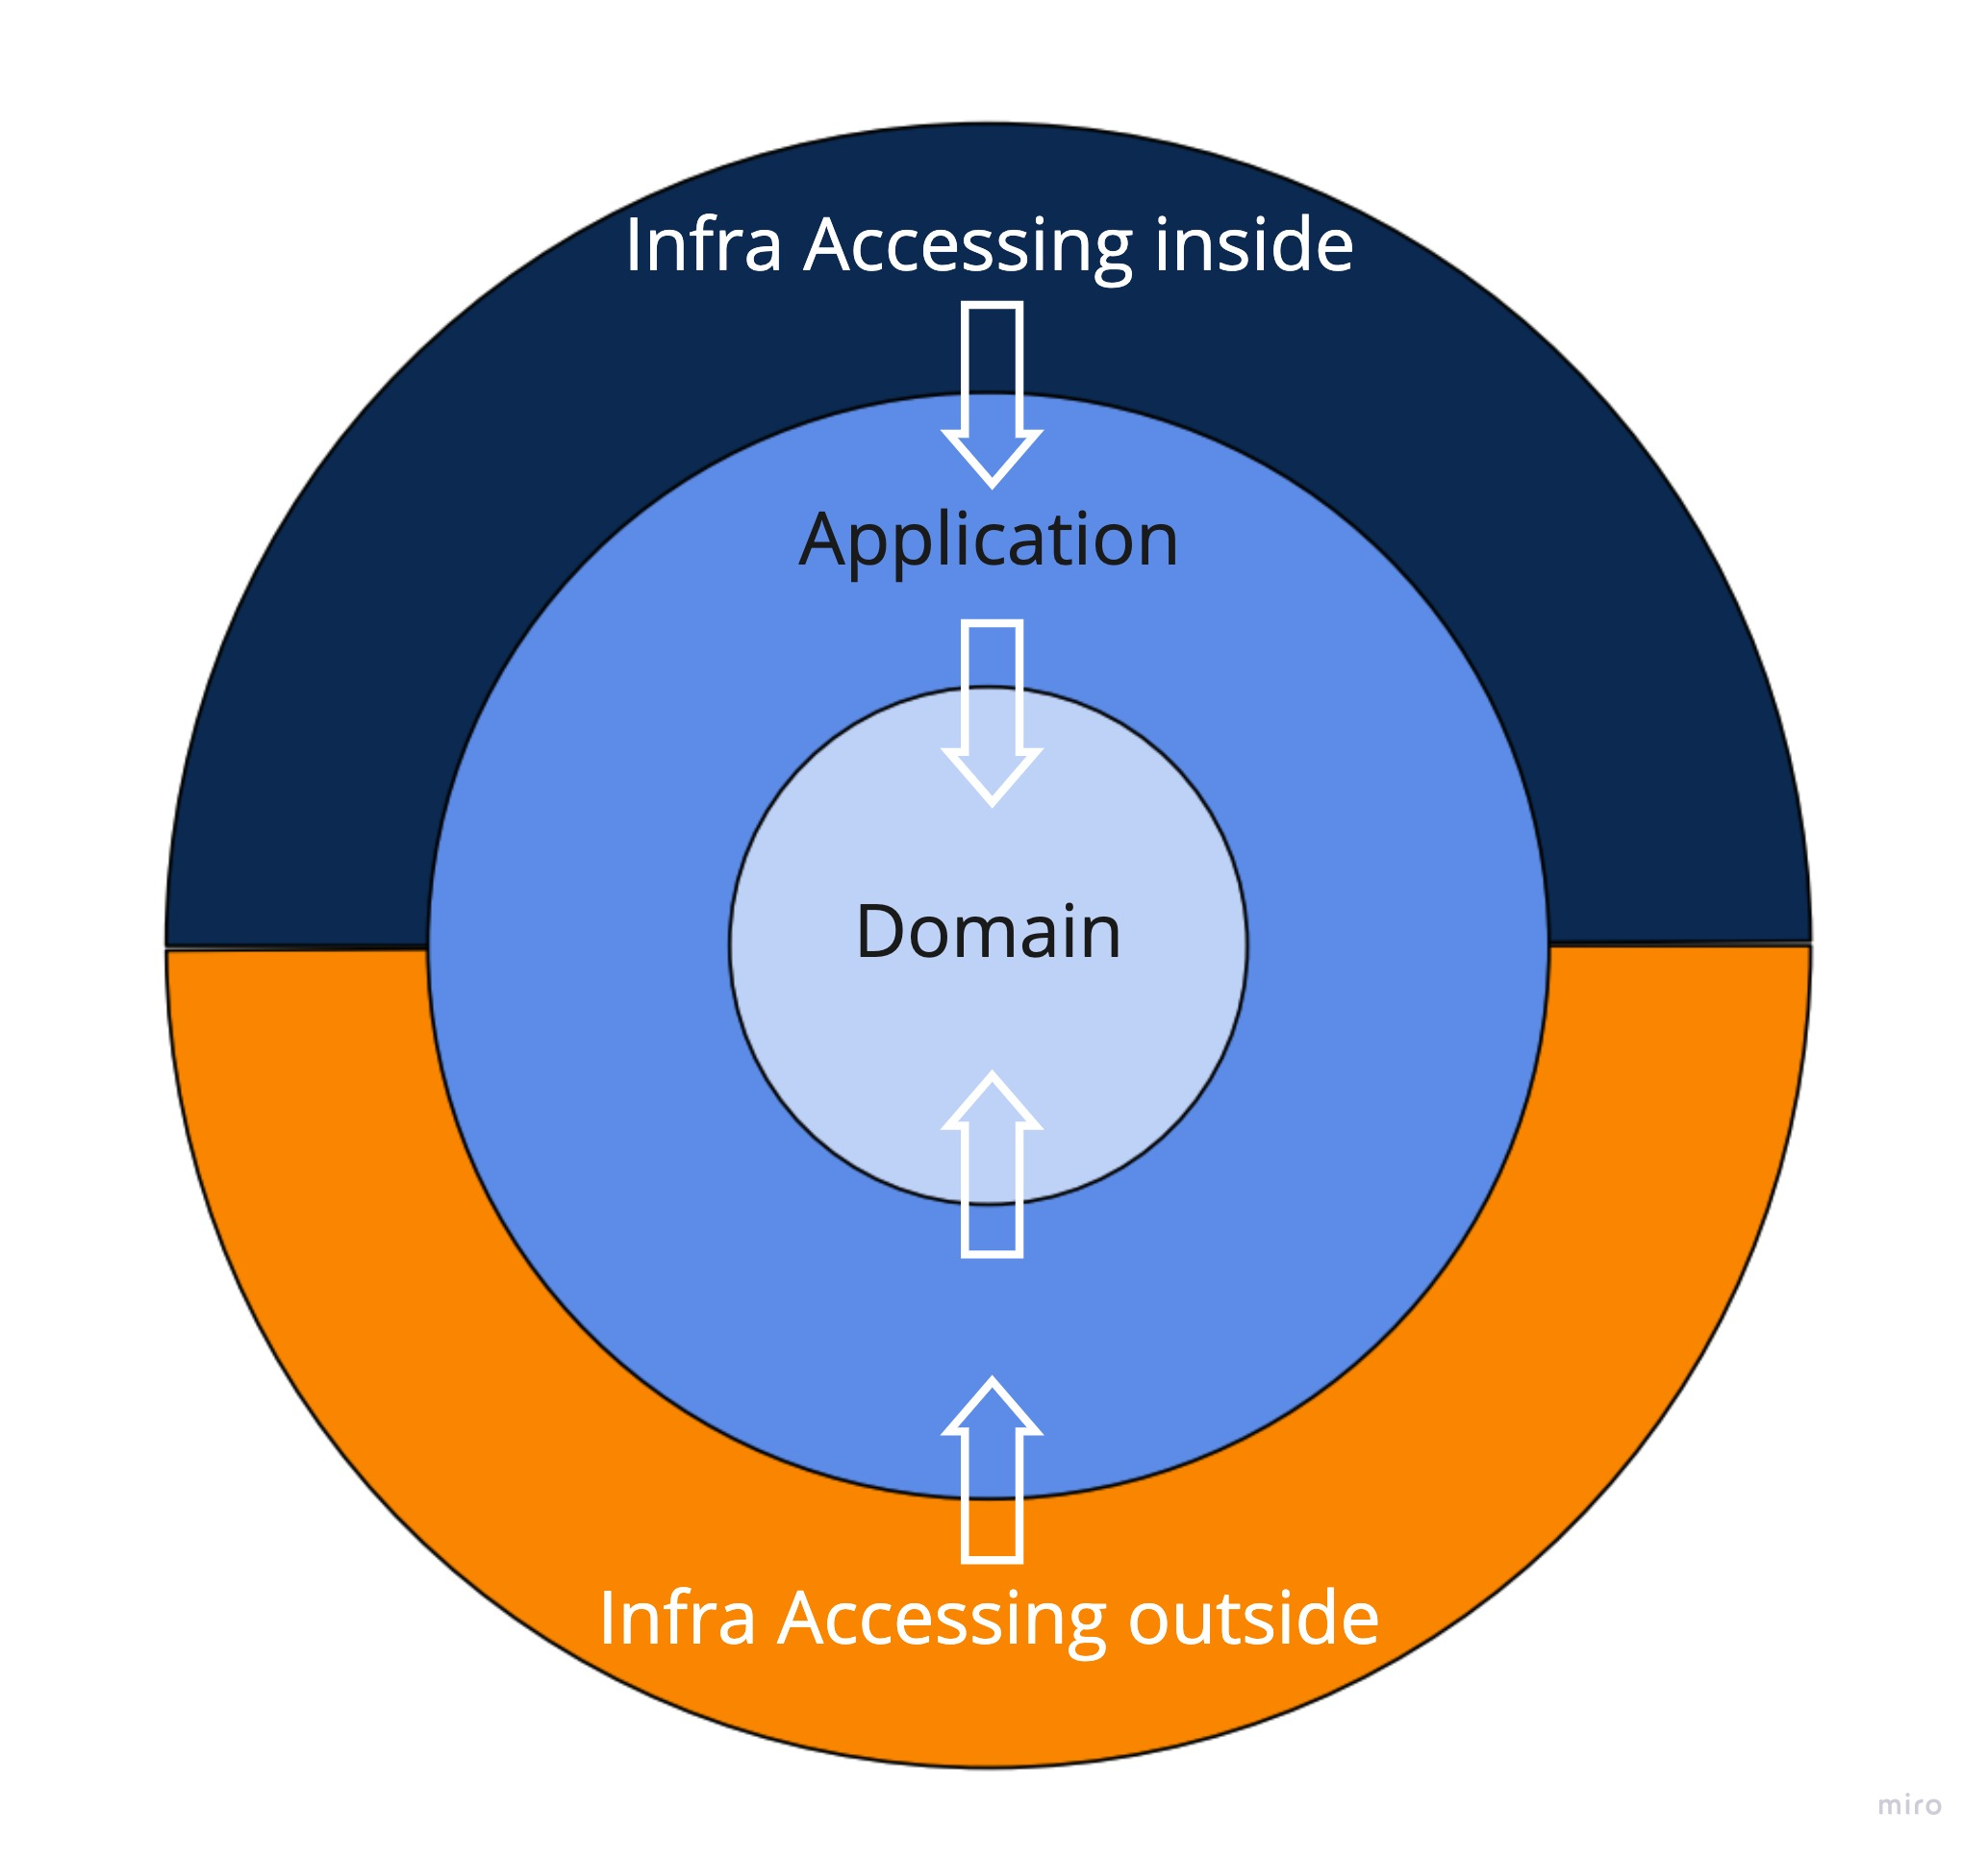
\includegraphics[height=0.3\textheight]{./part/Proyecto_ejecutivo/memoria_descriptiva/infoPreviaAntecedentes/img/PFM - Layer}
    \caption{layered architecture}\label{fig:layers}
\end{figure}

Una vez definidas las tres capas y resumido el concepto. Un punto importante a comentar es el concepto de la estrategia de mapping que hay entre capas. Cada capa requiere sus objetos de trabajo para estar desacoplada de las demás. Pero como en todo aspecto está sometido a discusión acerca de seguir la teoría a rajatabla y el pragmatismo de no verse envuelto en redundancias y sobredimensionar las soluciones.

En un extracto del libro Get Your Hands Dirty on Clean Architecture\cite{TomHombergs2019GYHD} podemos leer:
"\textit{ The argument might have gone something like this:}

\begin{itemize}
    \item \textit{Pro-Mapping Developer:}
    \subitem  \textit{> If we don’t map between layers, we have to use the same model in both layers which means that the layers will be tightly coupled!}
    \item \textit{Contra-Mapping Developer:}
    \subitem \textit{> But if we do map between layers, we produce a lot of boilerplate code which is overkill for many use cases, since they’re only doing CRUD and have the same model across layers anyways!}
\end{itemize}
\textit{As is often the case in discussions like this, there’s truth to both sides of the argument. Let’s discuss some mapping strategies with their pros and cons and see if we can help those developers make a decision.}"

Hay tantas estrategias como atajos dentro de este paradigma queramos asumir. Los tipos de mapping que se documentan en este libro:

\begin{itemize}
    \item The NoMapping Strategy \ref{fig:nomapping}
    \item The Two-Way MappingStrategy \ref{fig:twowaymapping}
    \item The Full MappingStrategy \ref{fig:fullmapping}
    \item The One-Way MappingStrategy \ref{fig:onWaymapping}
\end{itemize}

En todos estos casos vemos simplificado el dominio a una única entidad Account y vemos como separa dicho dominio del acceso al proceso que envía dinero a una cuenta y de dónde se guarda la información del envío de ese dinero.

\begin{figure}[H]
    \centering
    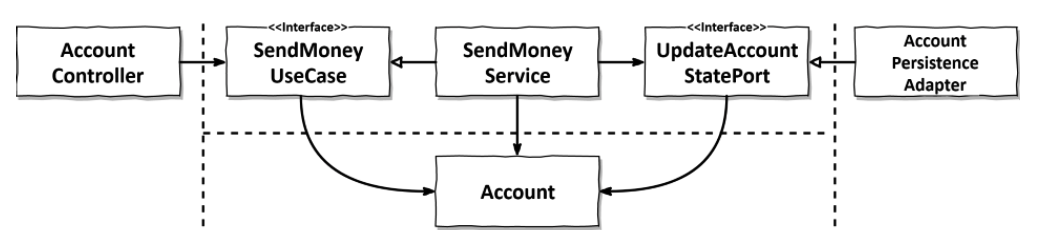
\includegraphics[height=0.1\textheight]{./part/Ejecucion/Seguimiento/CreateTaskUseCase/img/nomapping}
    \caption{No mapping strategy \cite{TomHombergs2019GYHD}}\label{fig:nomapping}
\end{figure}

\begin{figure}[H]
    \centering
    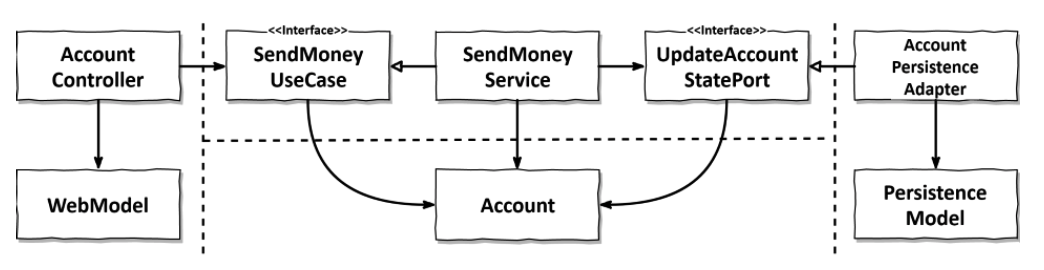
\includegraphics[height=0.1\textheight]{./part/Ejecucion/Seguimiento/CreateTaskUseCase/img/twowaymapping}
    \caption{two way mapping strategy \cite{TomHombergs2019GYHD}}\label{fig:twowaymapping}
\end{figure}

\begin{figure}[H]
    \centering
    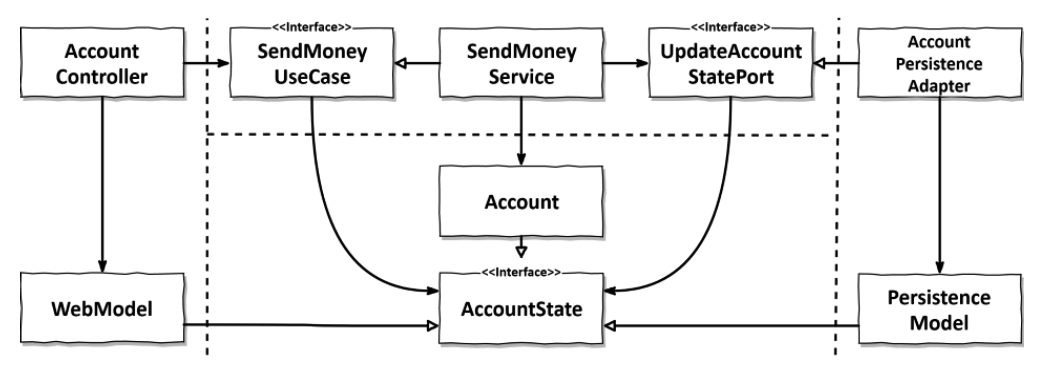
\includegraphics[height=0.1\textheight]{./part/Ejecucion/Seguimiento/CreateTaskUseCase/img/onWaymapping}
    \caption{One way mapping strategy \cite{TomHombergs2019GYHD}}\label{fig:onWaymapping}
\end{figure}

\begin{figure}[H]
    \centering
    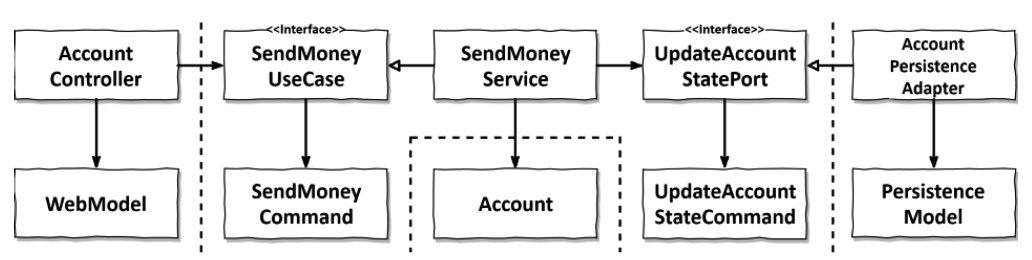
\includegraphics[height=0.1\textheight]{./part/Ejecucion/Seguimiento/CreateTaskUseCase/img/fullmapping}
    \caption{Full mapping strategy \cite{TomHombergs2019GYHD}}\label{fig:fullmapping}
\end{figure}


Todo programa creado en este proyecto(gestor de tareas, cliente y controlador) va a estar dividido por tanto en dichas capas y cada una tiene como objeto desarrollar un aspecto de la solución. Resumido de forma coloquial:

\begin{itemize}
    \item Dominio: responde a qué
    \item Aplicación: responde a cómo
    \item Infraestructura: responde a traves de qué
\end{itemize}

El concepto de CQRS



En un ejemplo rápido, si estamos manejando el concepto ¨Tarea¨ la definición de qué es una tarea es una cosa core, básica del programa diseñado. Lo que definamos como tarea tiene que ser estable, duradero. Cambiar mi definición de Tarea tocará la raiz de la solución que se presenta. Todo dependerá de qué consideremos una Tarea. Es por eso que lo llamamos Dominio. Todo debe depender del dominio y debe estar diseñado con cuidado. Abierto a añadir funcionalidades pero cerrado al cambio. Es decir podemos complementar la definición de tarea con una definición más completa y amplia, pero cambiar su significado es algo que invalidará tanto código que estaríamos hablando de otro software completamente nuevo.

Por ejemplo, si definimos tarea como un nombre y una fecha de comienzo. La tarea es un elemento de software que se compone de un campo para nombrarla y otro para guardar su valor:

Tarea: Hacer proyecto.
Fecha de comienzo: hoy.

y defino un programa que me dice la tarea más antigua. Si añadimos un campo nuevo con fecha de fin no rompemos nada. Añadimos funcionalidad al programa. Pero si decido que la fecha de comienzo no es importante elimino el campo y lo substituyo por esfuerzo necesario. he invalidado todo el concepto de tarea.

en el primer caso he definido Tarea como un concepto con fecha de inicio y en el otro la defino como algo que cuesta dias de esfuerzo. Por supuesto podría añadir en vez de sustituir. y de eso se trata. Definir qué es sobre lo que estamos hablando de forma esencial.

Siguiendo el mismo ejemplo Imaginemos que ya tenemos como dominio, concepto de Tarea, un elemento con nombre, fecha de inicio. Si queremos garantizar que no haya dos tareas el mismo día, antes de guardar esa tarea habremos de buscar si existe otra hoy y señalar al usuario si no puede introducir otra. Esto corresponde a una logica de la interacción entre los conceptos de dominio: las tareas se relacionan entre ellas bloqueando días, esto lo llamamos aplicación o capa de aplicación. antes de guardar hay que checkear que no existe otra hoy.

En pseudo código:
\begin{verbatim}
ComponenteDeAplicacion{

    CrearTareaHoy(nombre){
        if(!Dominio.HoyEstáLibre()){
            Error
        }
        Dominio.GuardarNuevaTarea(nombre)
    }
}
\end{verbatim}

\begin{itemize}
    \item Dominio(qué): las tareas se pueden crear
    \item Aplicación(cómo): comprobando que el día está libre
    \item Y  nos queda la última pregunta: a través de qué. Es decir a través de qué se comprueba que el día está libre y a través de qué tecnología se guarda?
\end{itemize}

La última pregunta es dónde se puede llegar a tender a emplear más minutos de investigación, configuración, desarrollo, discursiones y probablemente sea la más interesante desde un punto de vista puramente técnico. En este ejemplo: lo guardamos en una base de datos relacional, no relacional. escribimos el programa en un lenguaje en otro... Cómo va a ser el proceso de chequeo de fechas, guardamos en un formato, en otro, cuan eficiente es esa comprobación? cuando empezará a haber problema por el tamaño de la base de datos de cara a esa comprobación?

Todas esas preguntas son importantes e interesantes. Afectaran al precio de la solución, a la versatilidad o incluso a la viabilidad, pero desde un punto de vista empresarial o de ingeniería es un error a todas luces responder a esos problemas sin haber resuelto el problema de qué es lo que vamosa controlar y cómo lo vamos a controlar para poder presentarlo al cliente, venderlo, mejorar el diseño hasta que sea interesante para el cliente.

En una analogía a la construcción si un cliente te pide un espacio para almacenar, lo que hay que solucionar es el qué quieres guardar, cómo lo quieres guardar y no centrarse en cómo van a ser los cimientos, si la estructura va a ser de madera, metal o cemento, es un paso posterior. Si es carton y tienes que meter pales con un camión hay que centrarse en diseñar un espacio en el que no haya humedad, donde haya una zona de carga y descarga, un espacio para maniobra de los traspalés y una vez diseñada la solución ver qué materiales son los más adecuados para responder a esa solución: una nave industrial? un simple trastero? dependerá de la cantidad. Lo que intenta el análisis del Dominio y la aplicación es descubrir cuáles son las necesidades básicas, las funcionalidades básicas para poder evaluar una solución técnica adecuada.

El problema de la analogía es que es un poco contra-intuitivo porque el el software se va descubriendo (No se si meterme en dar valoracion de las diferencias entre el software y los productos fisicos de cara a ir descubriendo conforme programas)

El objetivo por tanto de este diseño que divide en estas tres capas es separar según los siguientes criterios

Hacer tabla de esto?
\begin{itemize}
    \item Dominio:          tendencia al cambio baja    dependencia a software nula*)    Interacción con No tecnicos alta
    \item Aplicación:       tendencia al media          dependencia a software externo nula* Interacción con No tecnicos alta
    \item Infraestructura:  tendencia al alta           dependencia a software  Interacción con No tecnicos baja
\end{itemize}

Del dominio se acaba hablando con los managers, comerciales, clientes y es un lenguaje comun a toda la compañía, se suele tner que hacer diagramas, gráficos, dosieres de ello. Si no está separado tiene a ocultarse entre detalles técnicos, se vuelve dificil de explicar qué es lo que se está manejando y cómo funciona. Degenera.

Falta un dejalle en nuestro ejemplo de tarea. No es pequeño

\begin{verbatim}

ComponenteDeAplicacion{

    CrearTareaHoy(nombre){
        if(!Dominio.HoyEstáLibre()){
            Error
        }
        Dominio.GuardarNuevaTarea(nombre)
    }
}

\end{verbatim}


es la comprobación de que el día está libre tan importante en nuestro software que no es una forma de interaccionar de las tareas
si no un requisito indispensable? lo que no estamos preguntando es si es parte del dominio o es una simple funcionalidad de Crear la tarea hoy. Por ejemplo veamos este codigo

Supongamos que consideramos tan importante esta comprobación que pasamos la comprobación dentro de la funcion GuardarTareaNueva de domino para que nadie pueda crear una tarea en ninguna parte del codigo en un dia ocupado por error. Imaginamos que llega otra funcionalidad de crear tareas en otros dias que no sean hoy y abrimos funcionalidad pero no la cambiamos, podemos modificar nuestro codigo de crear tarea hoy para que pase la fecha de hoy pero permitir que se cree otra funcion que permita pasar otra fecha.

\begin{verbatim}
ComponenteDeAplicacion{

    CrearTareaHoy(nombre){
        Dominio.GuardarNuevaTarea(nombre,hoy)
    }

    CrearTareaEnFecha(nombre,fecha){
        Dominio.GuardarNuevaTarea(nombre,fecha)
    }
}

\end{verbatim}

Suponiendo que dominio.guardarTarea ya hace la comprobación siempre


Ahora planteemos que llega el cliente y quiere tener la posibilidad de crear dias saturados de tareas pero seguir pudiendo crear tareas con la seguridad de que no hay más tareas ya no podriamos hacer esto:

\begin{verbatim}

ComponenteDeAplicacion{

    CrearTareaHoy(nombre){
        Dominio.GuardarNuevaTarea(nombre,hoy)
    }

    CrearTareaEnFecha(nombre,fecha){
        Dominio.GuardarNuevaTarea(nombre,fecha)
    }

    CrearTareaHoyAunqueHayaMas(nombre){
        -->>> Dominio.GuardarNuevaTarea(nombre) // No funcionaria
    }

}
\end{verbatim}

porque Dominio.GuardarNuevaTarea ya hace la comprobación por dentro. Decidir cómo funciona el dominio.

Decidir qué partes son de aplicación y qué partes son de dominio es una tarea continua. No es fácil discernirlo en todos los casos. Y es por esto que esta división cobra todavía más sentido. Qué cosas se meten en dominio o se sacan aplicación es una tarea constante y compleja que si mezclamos con la infraestructura no nos deja ver esta cosas de forma rápida y clara.

Por supuesto podriamos crear dos funciones de dominio

GuardarNuevaTareaComprobando()
GuardarNuevaTareaSinComprobar()

precisamente ahí está el tema. En ir definiendo el dominio de forma que se pueda ampliar la funcionalidad pero que no se tenga que reescribir la funcionalidad.

El ejemplo de un proceso para no sufrir en estos cambios seria

V0

\begin{verbatim}
ComponenteDeAplicacion{

    CrearTareaHoy(nombre){
        if(!Dominio.HoyEstáLibre()){
            Error
        }
        Dominio.GuardarNuevaTarea(nombre)
    }
}

Dominio{
    Dominio.GuardarNuevaTarea(nombre)
}

\end{verbatim}

V1

\begin{verbatim}
ComponenteDeAplicacion{

    CrearTareaHoy(nombre){
        Dominio.GuardarNuevaTareaComprobandoFecha(nombre,hoy)
    }

    CrearTareaEnFecha(nombre,fecha){
        Dominio.GuardarNuevaTareaComprobandoFecha(nombre,fecha)
    }
}


Dominio{
    Dominio.GuardarNuevaTarea(nombre)
    Dominio.GuardarNuevaTareaComprobandoFecha(nombre,fecha){
        if(!Dominio.HoyEstáLibre()){
            Error
        }
        Dominio.GuardarNuevaTarea(nombre)
    }
}

\end{verbatim}

V3

\begin{verbatim}

ComponenteDeAplicacion{

    CrearTareaHoy(nombre){
        Dominio.GuardarNuevaTareaComprobandoFecha(nombre,hoy)
    }

    CrearTareaEnFecha(nombre,fecha){
        Dominio.GuardarNuevaTareaComprobandoFecha(nombre,fecha)
    }

    CrearTareaHoyAunqueHayaMas(nombre){
        Dominio.GuardarNuevaTarea(nombre,fecha)
    }
}


Dominio{
    Dominio.GuardarNuevaTarea(nombre)
    Dominio.GuardarNuevaTareaComprobandoFecha(nombre,fecha){
        if(!Dominio.HoyEstáLibre()){
            Error
        }
        Dominio.GuardarNuevaTarea(nombre)
    }
}
\end{verbatim}

Lo importante, y por lo que se expone un ejemplo de este proceso es que se puede apreciar que en el descubrimiento del codigo final se esta hablando en terminos llanos, entendibles por todo el mundo sobre como funcionan las cosas, es un proceso en el que interviene todo el equipo-empresa. Que se discute cómo tienen que funcionar las cosas. En tener controlada esta parte es donde se garantiza la calidad. Veremos muchos ejemplos de decisiones de division applicacion-dominio en la memoria descriptiva

luego en la descripcion del proceso de ejecucion podremos ver cambios en estas decisiones conforme se va desarrollando la solución y cómo haber definido esta división y estructura ayuda a la gestion-comprension-documentación y llegada a buen puerto de la funcionalidad del software.


Una vez descrito qué son las capas tenemos que explicar qué elementos podemos encontrar en ellas:


Dominio

Entity
VO
AggregateRoot
Dto
Service
Repository

Applicacion

Command
Query
EventHandler
UseCase


El bloque funcional más básico a nivel conceptual dentro del domino es \textit{Entity}. Una entity compuesta de más entites se vuelve un agregate root. De forma genérica Para cada entity-aggregateRoot existirá una estructura de archivos tal como en el diagrama de estructura de archivos \ref{fig:folderEntity}

\begin{figure}[h]
    \dirtree{%
        .1 Domain.
        .2 EntityName.
        .3 Entity.go.
        .3 ValueObject.go.
        .3 SubEntityComponent.
        .4 SubEntityComponent.go.
        .4 ValueObject.go.
        .3 Finder.go.
        .3 Recorder.go.
        .3 Eraser.go.
    }\caption{}
    \label{fig:folderEntity}
\end{figure}

El objetivo de esto es que simplemente leyendo el nombre de los archivos ya estás entiendiendo el sistema.

Conceptualmente el estará concebido en capas. Las capas cuanto más profundas sean menos tenderán a cambiar, seran las bases del proyecto y de lo que depende todo lo demas. si hay cambios en las capas superiores no afectaran al interior. Si hay cambios en el interior afectarán a todo, es por esto que el diseño del interior se concibe como Dominio de la aplicación llamado DDD.

en el proceso iterativo del desarrollo hay partes que van quedando más rígidas al estar más definidas. Todo se acopla a ello eso es el dominio. Es por esto que cuando empiezas a desarrollar conceptos nuevos puede ser necesario implementarlo en aplicación mientras se va viendo claro y luego refactorizar para incluirlo en el dominio una vez está claro.
Veamos un ejemplo:

\begin{figure}[H]
    
\dirtree{%
    .1 Project .
        .2 Adapter.
            .3 in.
                .4 Http.
                .4 GRPC.
            .3 out.
                .4 Mysql.
                .4 GRPC.
        .2 Application.
            .3 Port.
                .4 in.
                    .5 <Domain Concept>.
                        .6 UseCase.
                            .7 SomeCommands.
                                .8 Command.
                                .8 CommandUseCase.
                            .7 SomeQuery.
                                .8 Query.
                                .8 QueryUseCase.
                            .7 SomeEventHandler.
                                .8 Event.
                                .8 EventUseCase.
                .4 out.
                    .5 External out interactions.
        .2 Domain.
            .3 EntityName.
}\label{directoryStructure}
    \caption{}
    \label{fig:ProjectfolderStructure}
\end{figure}

En realidad toda estructura es para que visualmente se entienda como está concebido el proyecto. nuestro objetivo siempre tiene que ser que no haya imports (dependencias) de paquetes de fuera hacia adentro


para entender mejor el objetivo de estas capas podemos entenderlas de forma más simple como lo que lo que hay más en la superficie es lo que más grado de incertidumbre tiene, es decir, lo que más expuesto al cambio está. por lo tanto queremos separarlo lo máximo posible del código que si está cerrado al cambio y abierto sólo a la extensión. No hay que confundirlo tanto con el principio OpenClose que siempre se aplica en toda la aplicación si no como lo que es susceptible de quedar como codigo muerto, inservible, con mala sintaxis debido al desconocimiento de librerias.

Por orden sabemos que la capa de adapter donde vamos a investigar acerca de GRPC, donde no sabemos ni la librería que vamos a utilizar, Mysql donde tenemos que escoger un paquete de ORM entre todos los disponibles en el mercado opensource. Es seguro que habrá elecciones de estas herramientas que después de estudiadas no respondan a nuestras espectativas y quede como linea futura su sustitución. Este es el devenir inevitable y típico de un software, para no deshechar partes del código que sí sean reutilizables o estén completamente terminadas nos desacoplamos de estos puntos calientes. Más aún siendo un proyecto con un tiempo muy limitado y queriendo despejar dudas en muchos frentes com prioridad versus a la perfección se va a optar en muchas ocasiones por dejar código funcional sin ninguna atención a la calidad, esto ocurre en todos los proyecctos con deadlines ajustados. Esta filosofia nos proteje y ayuda a usar la rapidez sin sacrificar la estabilidad y dejando la suciedad sólo en los puntos que no son críticos.


Un punto interesante de esta estructura son los Application port out. En qu'e se diferencia del recorder de dominio por ejemplo que es una interfaz de un adaptador de salida a base de datos. Pongamos por ejemplo que cuando se crea una Entity hay un concepto core de dominio que sea lanzar un evento entityNameCreated. No queremos bajo ningún concepto que la lógica de crear la Entity y que se lance el evento quepa la posibilidiad de ejecutarse por separado o de ejecutarse una pero no otra. Es por esto que está dentro de dominio y para ello crearemos un Recorder service que haga uso del Recorder y esté junto la creacion y el lanzamiento del evento. Haciendo el recorder interface privado y solo exponiendo el RecorderService de tal forma que no se pueda usar por separado.

Ahora imaginemos que tenemos el siguiente caso de uso:
Cada vez que se crea una Entity mediante GRPC queremos puntualmente que si la entity Tiene un campo name este sea \textit{ejemplo} entonces se envíe un correo electrónico avisando a administración de que se ha creado una entity con dicho name.
pero si se crea mediante terminal significa que lo está haciendo la propia administración y por tanto el correo no es necesario. Si en el Dominio Recorder implementamos la lógica de enviar siempre el correo no podríamos evitarlo, además de que no es un concepto de consistencia de dominio. si no se enviara el correo los datos son validos. si quisieramos meterlo en dominio tendríamos que enviar la información de quién lo está creado para saber si mandar el correo o no haciéndo la lógica más compleja y difusa por algo que en realidad no trata de la consistencia de la aplicación si no de un caso de uso en concreto. En este caso creariamos un Port.Out.Email.EmailSenderOnCreation(name) y lo implementariamos en los adaptadores de salida donde configuraríamos el correo de administración. este puerto de salida sería utilizado en el puerto de entrada de grpc Create

\begin{figure}[H]
    
\dirtree{%
    .1 Project .
        .2 Adapter.
            .3 in.
                .4 GRPC.
                    .5 CreateEntityGrpcCall.
                .4 Console.
                    .5 CreateEntityTerminalCommand.
            .3 out.
                .4 Email.
                    .5 SendEmailOnCreationImplementation (*1).
                .4 Mysql.
                    .5 SaveEntityImplementation (*2).
        .2 Application.
            .3 Port.
                .4 in.
                    .5 Entity.
                        .6 CreateUseCase.
                            .7 CreateCommand.
                                .8 CreateCommand (using sendEmail param in this example).
                                .8 CreateUseCase.
                            .7 SomeEventHandler.
                                .8 CreationEvent.
                                .8 CreationEventUseCase.
                .4 out.
                    .5 Email.
                        .6 SendEmailConCreation (interface for *1).
        .2 Domain.
            .3 Entity.
                .4 EntityName.go.
                .4 RecorderService.go (using Recorder.go and ensuring to raise CreationEvent together with the recording).
                .4 recorder.go (interface for *2).
}\label{directoryStructureOut}
    \caption{}
    \label{fig:ProjectfolderStructurePortOut}
\end{figure}